\documentclass[30pt,twocolumn,letterpaper]{article}
\usepackage{cvpr}
\usepackage{times}
\usepackage{booktabs}
\usepackage{epsfig}
\usepackage{graphicx}
\usepackage{amsmath}
\usepackage{amssymb}
\cvprfinalcopy
\def\cvprPaperID{****}
\def\httilde{\mbox{\tt\raisebox{-.5ex}{\symbol{126}}}}
\usepackage{graphicx}
\usepackage{indentfirst}
\setlength{\parindent}{2em}
\usepackage{cite}
\usepackage[colorlinks,linkcolor=red,anchorcolor=blue,citecolor=green,backref=page]{hyperref}
\author{Qilei Zhang\\\\
Jun 18 2018}
\title{Decoupled Neural Interfaces Using Synthetic Gradients}
\begin{document}
\maketitle
\begin{abstract}
  Training directed neural networks typically requires forward-propagating data through a computation graph, followed by backpropagating error signal, to produce weight updates. All layers, or more generally, modules, of the network are therefore locked, in the sense that they must wait for the remainder of the network to execute forwards and propagate error backwards before they can be updated.
\end{abstract}
\section{Introduction}
Each layer (or module) in a directed neural network can be considered a computation step, that transforms its incoming data. These modules are connected via directed edges, creating a forward processing graph which defines the flow of data from the network inputs, through each module, producing network outputs.\cite{Krogh1995Neural}. \\
\begin{figure}[htbp]
\small
\centering
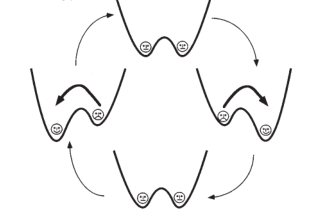
\includegraphics[width=20em]{000.png}
\caption{General communication protocol between A and B. After
receiving the message hA from A, B can use its model of A,
MB, to send back synthetic gradients ?��A which are trained to approximate
real error gradients ��A. Note that A does not need to
wait for any extra computation after itself to get the correct error
gradients, hence decoupling the backward computation. The
feedback model MB can also be conditioned on any privileged information
or context, c, available during training such as a label}
\label{fig:lable}
\end{figure}\\
\begin{equation}
\quad x'(t)=-V'(x)+A_0cos(wt+o)+u(t)
\end{equation}
\section{Decoupled Neural Interfaces}
We begin by describing the high-level communication protocol that is used to allow asynchronously learning agents to communicate\cite{Pustejovsky1998The}. This protocol allows A to send messages to B in a way that A and B are update decoupled �C A does not have to wait for B to evaluate the true utility\cite{Sanger1989Optimal} before it can be updated �Cand A can still learn to send messages of high utility to B.\\
\begin{figure}[htbp]
\small
\centering
\includegraphics[width=20em]{001.png}
\caption{Completely unlocked feed-forward network training allowing forward and update decoupling of layers.}
\label{fig:lable}
\end{figure}\\
\section{Conclusion}
In this work we introduced a method, DNI using synthetic gradients, which allows decoupled communication between components\cite{Szu1992Neural}, such that they can be independently updated.\cite{Wittrock1989Generative}.
{\small
\bibliographystyle{ieee}
\bibliography{1}
}
\end{document}
